\chapter{Results and discussion}

\section{Data exploration}
As described earlier in Chapter 3, the data for the experiments is from Twitter. It was extracted and pre-processed by \cite{preotiuc-pietro_automatically_2019} and further enhanced with the labels for complaint severity by \cite{jinModelingSeverityComplaints2021}. What follows are the key findings from the exploratory data analysis performed. Additionally, some minor differences in the distribution of the tweets across the domains are observed between the latest version of the dataset available in the public domain\footnote{\url{https://archive.org/details/complaint_severity_data}} and the distribution described in the original paper. Since the variations are minor (0.5 to 2\%), any potential impact on the model performance should be insignificant in the context of the objectives of the experiments.


\begin{figure}[htb]
    \centering
    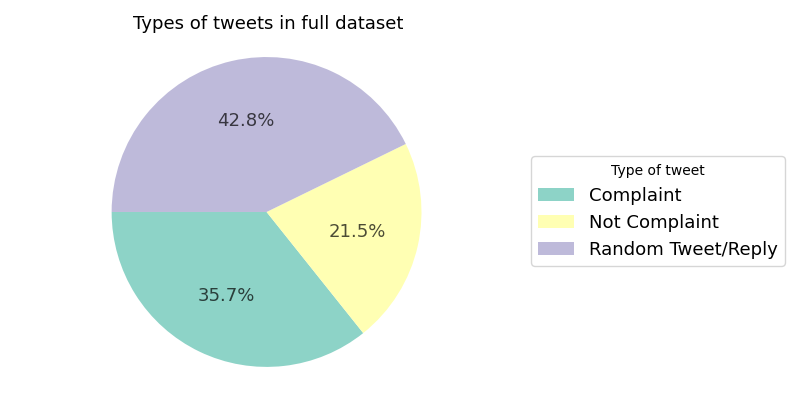
\includegraphics[width=9cm]{figures/compl_non_random_dist.png}
    \vspace*{-3mm}
    \caption{Illustrates the distribution of tweets categorised as 'complaints' and 'not complaints', with random 'tweets / replies' shown separately.}
    \label{fig: compl_non_random_dist}
\end{figure}


All tweets categorised as complaints are assigned the label \texttt{label:1}, while tweets that do not constitute complaints are assigned \texttt{label:0}. In terms of class distribution, the dataset is skewed towards 'not complaint' tweets, as depicted in Figure \ref{fig: compl_non_random_dist}, where \texttt{label:1} represents 35.7\% and \texttt{label:0} represents 64.3\% of the dataset. To ensure a more representative dataset, the authors of \cite{preotiuc-pietro_automatically_2019} introduced several random tweets and replies. This approach aligns with the real-world scenario where complaint-related posts form a smaller proportion within an organization's social media tweets and posts. Additionally, this strategy has the potential to enhance the model's ability to generalize effectively during the finetuning process.\\

\begin{figure}[htbp]
    \centering
    \captionsetup{font=small}
    \begin{subfigure}{0.49\textwidth}
        \centering
        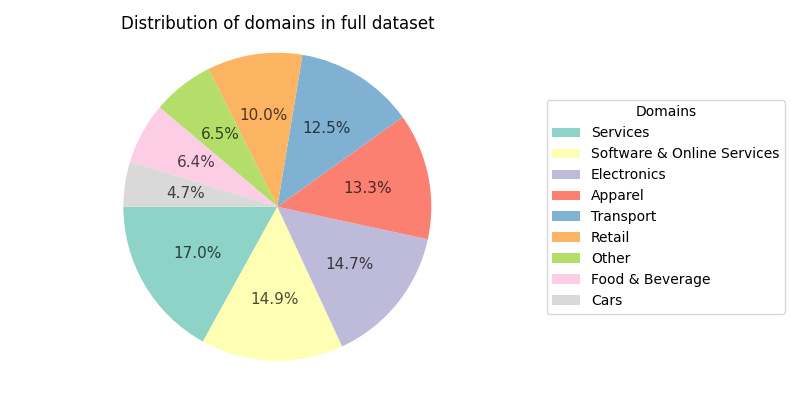
\includegraphics[width=\linewidth]{figures/domain_dist.png}
        \caption{Proportion of each domains}
        \label{fig: domain_dist_pct}
    \end{subfigure}
    \hfill
    \begin{subfigure}{0.49\textwidth}
        \centering
        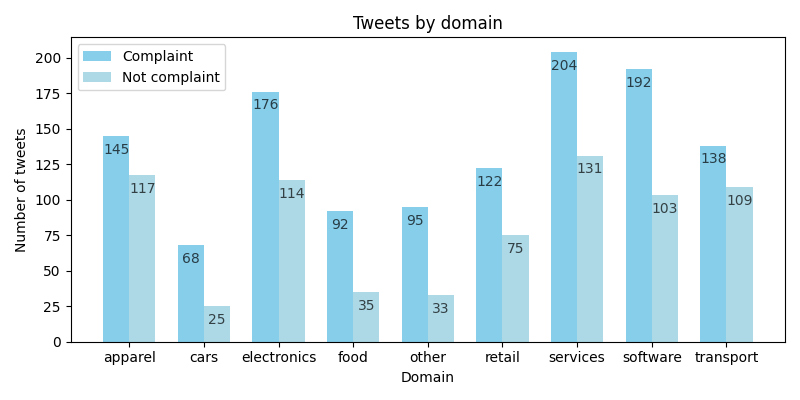
\includegraphics[width=\linewidth]{figures/domain_counts_bar_norandom.png}
        \caption{No. of tweets for each domains}
        \label{fig: domain_dist_count}
    \end{subfigure}
    \caption{Shows the distribution of the domains used in the dataset}
    \label{fig: compl_main_dist}
\end{figure}

\section{Comparision of model performance}
**TO UPDATE**

\section{Analysis of best performing model}
**TO UPDATE**

\section{Cross-domain results}
**TO UPDATE**